\section{Results and Discussion} \label{sec:results}


\begin{figure*}
  \centering

\begin{subfigure}[b]{\textwidth}
\centering
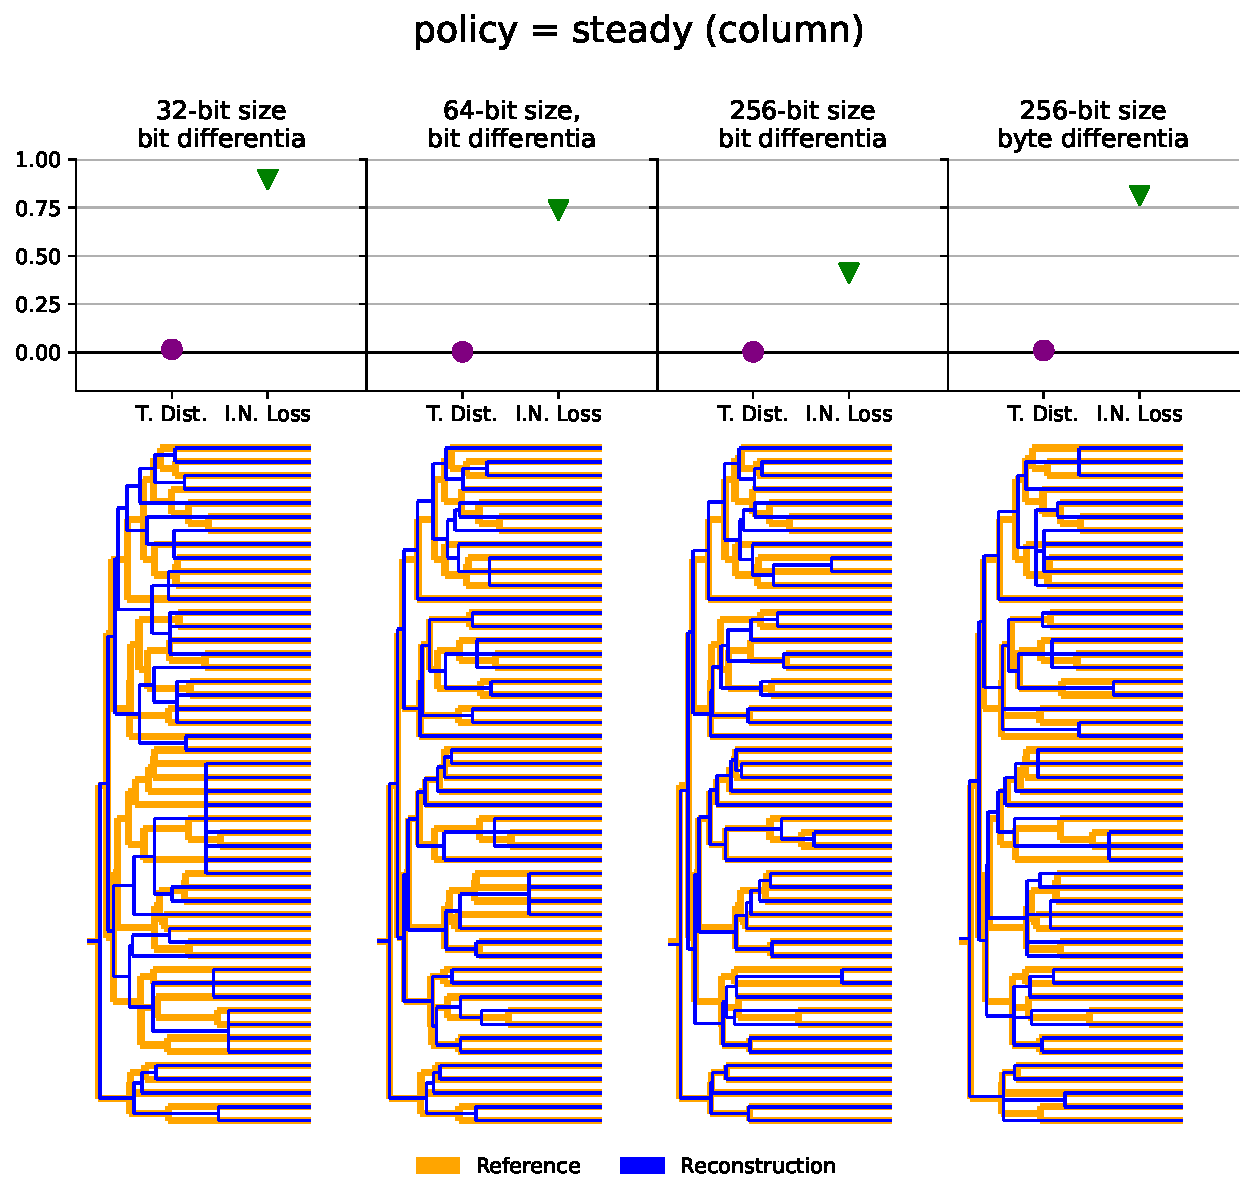
\includegraphics[width=0.5\textwidth]{binder/binder/outplots/a=examplepanel+policy=col-steady+regime=drift+ext=}%
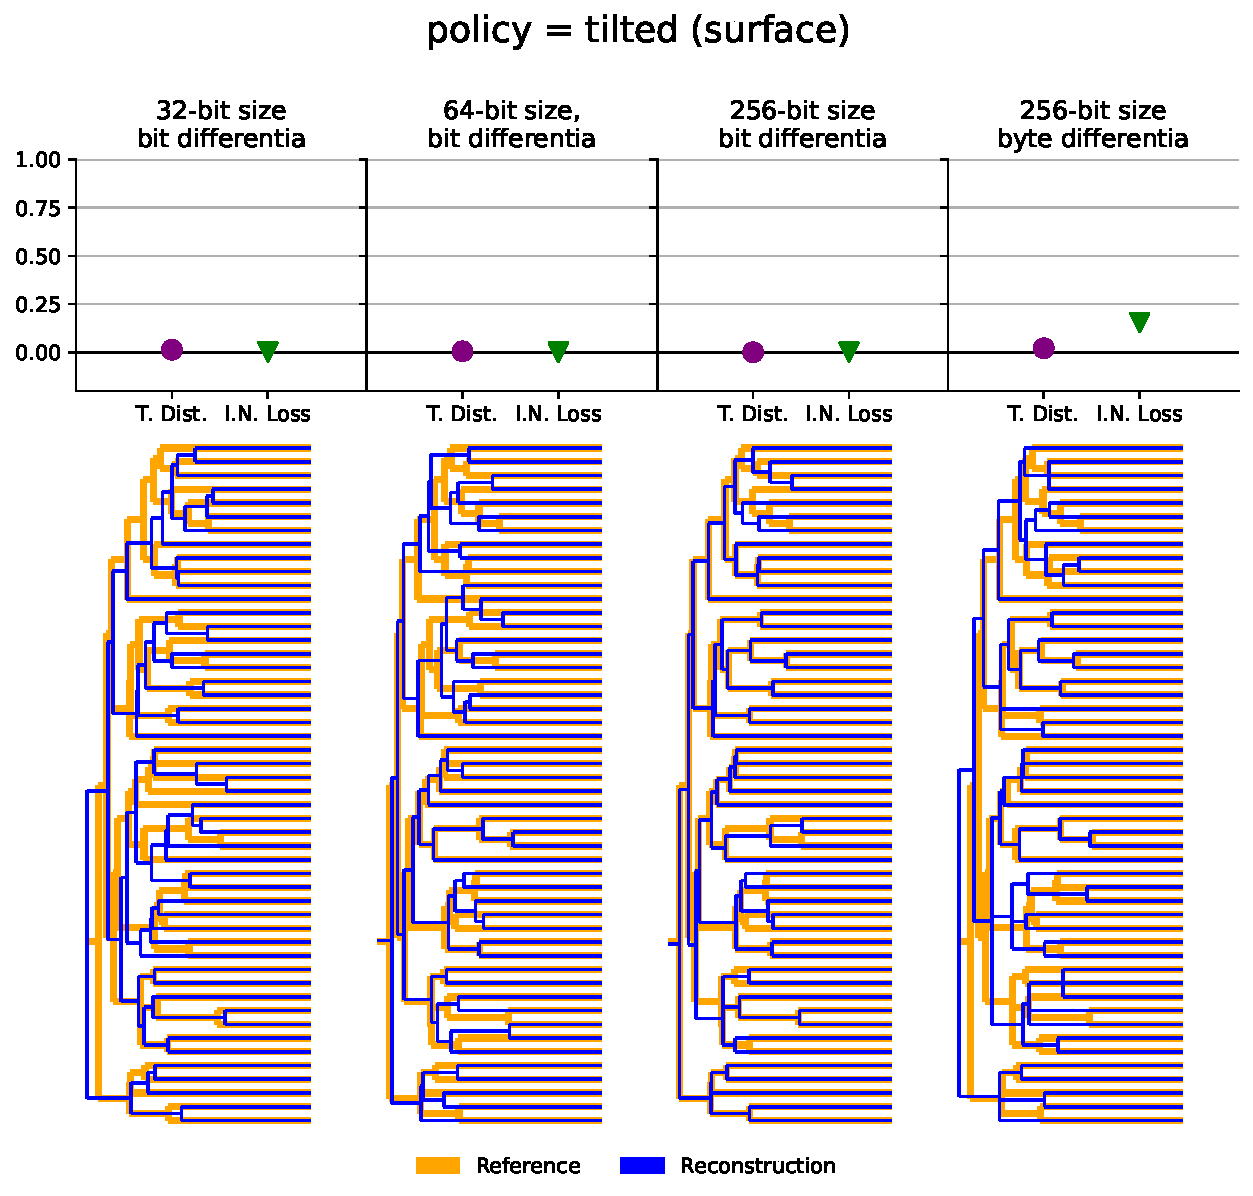
\includegraphics[width=0.5\textwidth]{binder/binder/outplots/a=examplepanel+policy=surf-tilted+regime=drift+ext=}
\caption{drift regime --- high phylogenetic richness}
\label{fig:examplepanel-drift}
\end{subfigure}

\begin{subfigure}[b]{\textwidth}
\centering
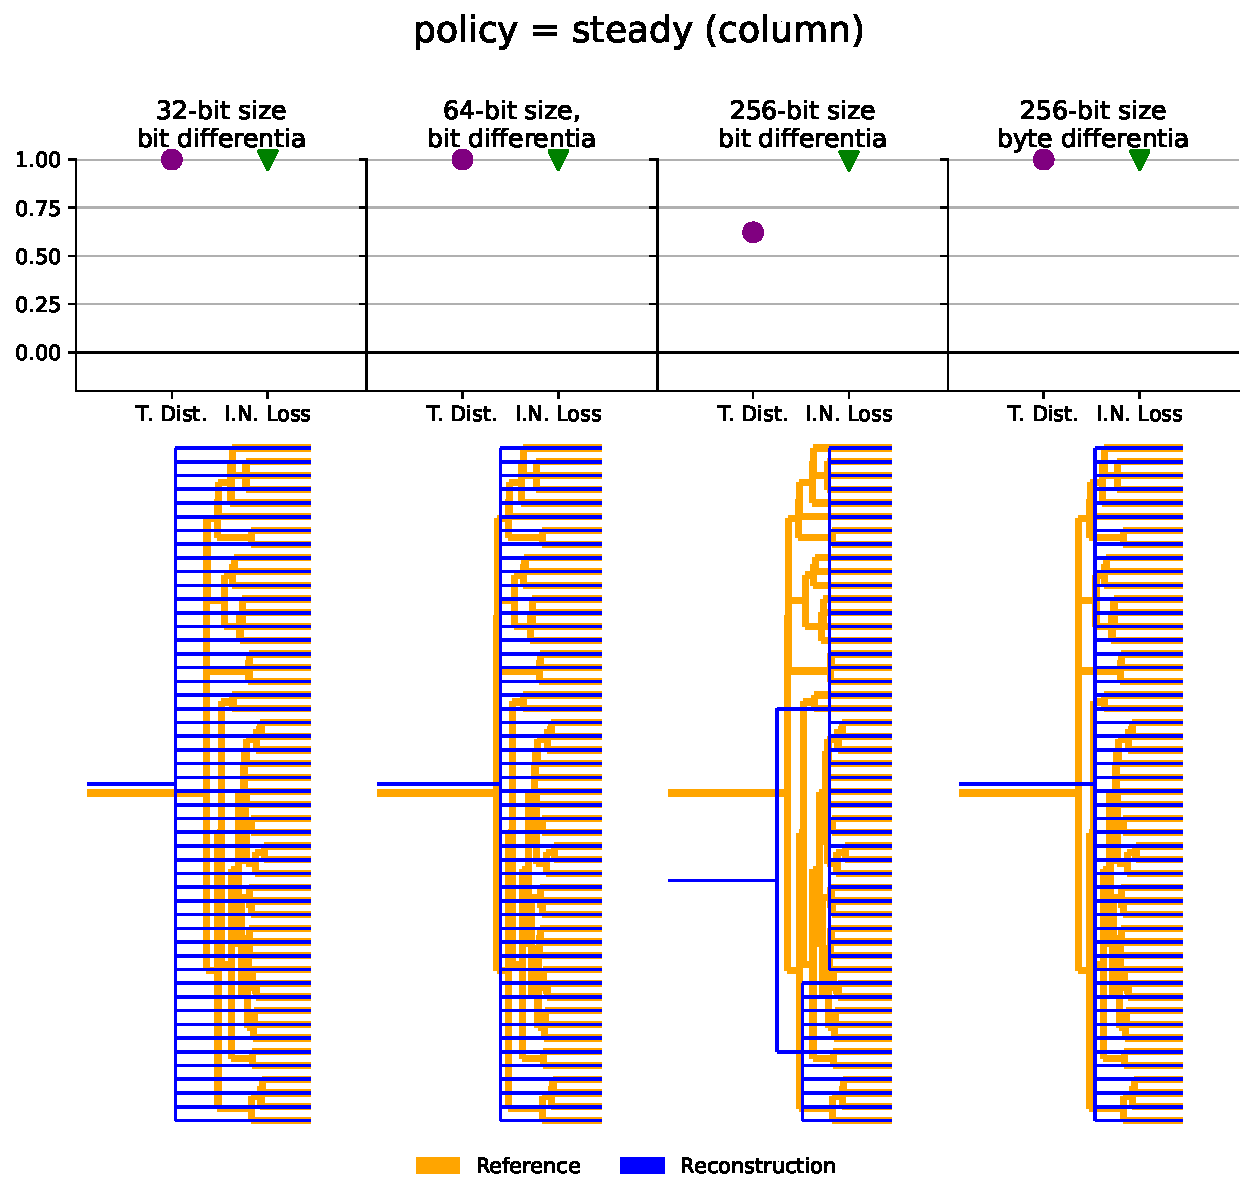
\includegraphics[width=0.5\textwidth]{binder/binder/outplots/a=examplepanel+policy=col-steady+regime=plain+ext=}%
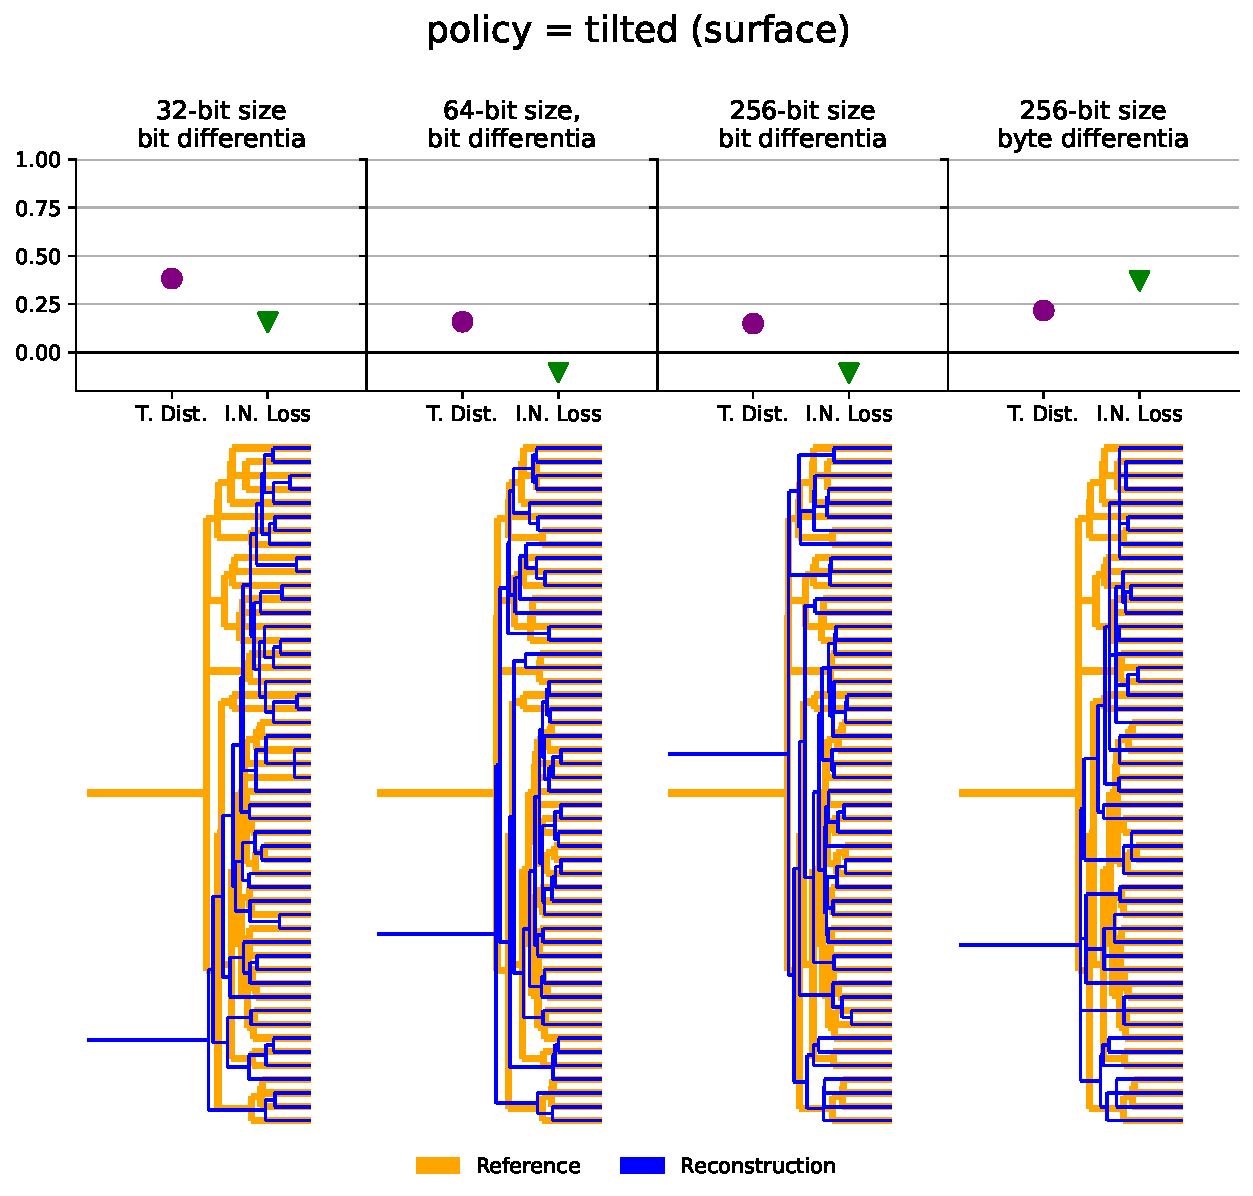
\includegraphics[width=0.5\textwidth]{binder/binder/outplots/a=examplepanel+policy=surf-tilted+regime=plain+ext=}
\caption{plain regime --- low phylogenetic richness}
\label{fig:examplepanel-plain}
\end{subfigure}

  \caption{%
  \textbf{Reconstruction vs. Reference Examples.}
  Comparison of reconstruction to reference tree for steady and tilted policies under drift (\ref{fig:examplepanel-drift}) and plain (\ref{fig:examplepanel-plain}) evolutionary regimes.
  Panel tops show reconstruction quality metrics and panel bottoms overlay reconstruction (blue) on reference tree (orange). 
  Phylogeny time axes are log scale.
  Note that overlay layout is naive, so can underrepresent agreement between trees; however, comparison is informative to general differences in tree structure.
  }
  \label{fig:examplepanel}

\end{figure*}


\begin{figure*}
  \centering
    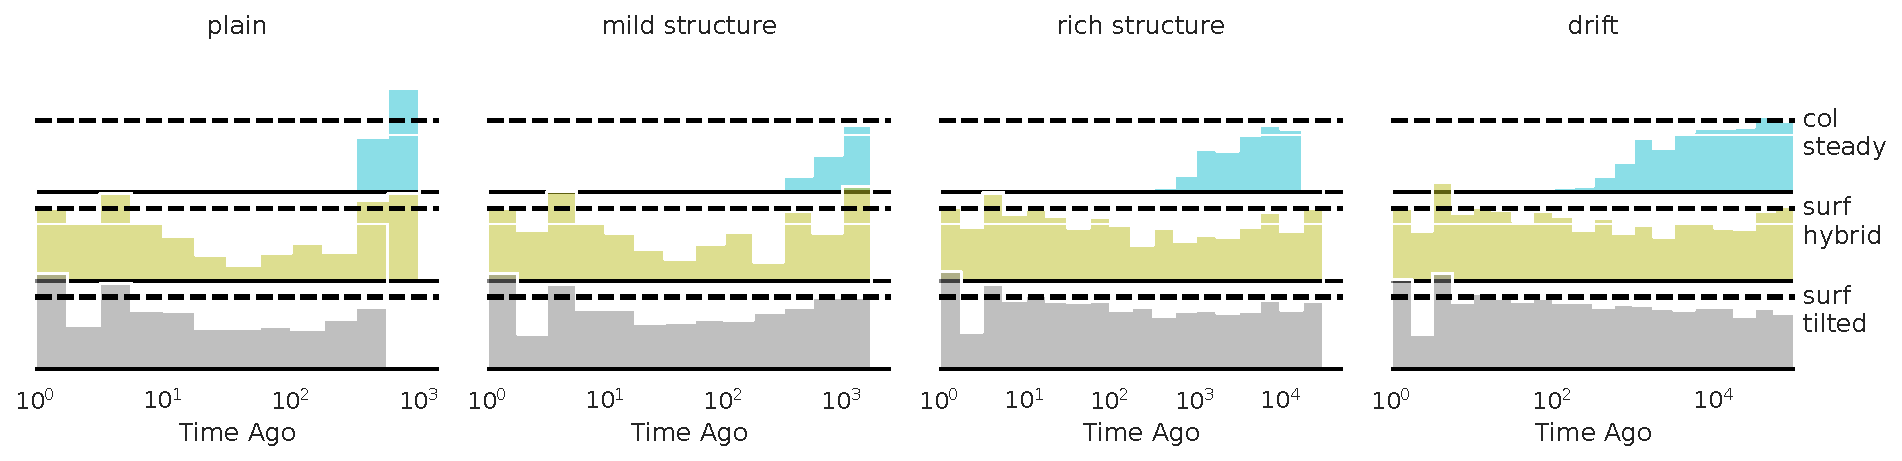
\includegraphics[width=\linewidth]{binder/binder/teeplots/annotation-size-bits=256+col=scenario+differentia-width-bits=8+hue=kind+row=algo+scale=npop65536-ngen100000+viz=joyhist+x=time-ago+ext=}
\caption{%
  \textbf{How does phylogeny structure differ by retention policy?}
  reconstruction node densities; 256-bit size, byte differentia
  TODO
}
  \label{fig:recency-structure}

\end{figure*}


\subsection{Surface vs. Column} \label{sec:surface-vs-column}

\begin{figure*}
  \centering
  \begin{subfigure}[b]{0.5\textwidth}
    \centering
    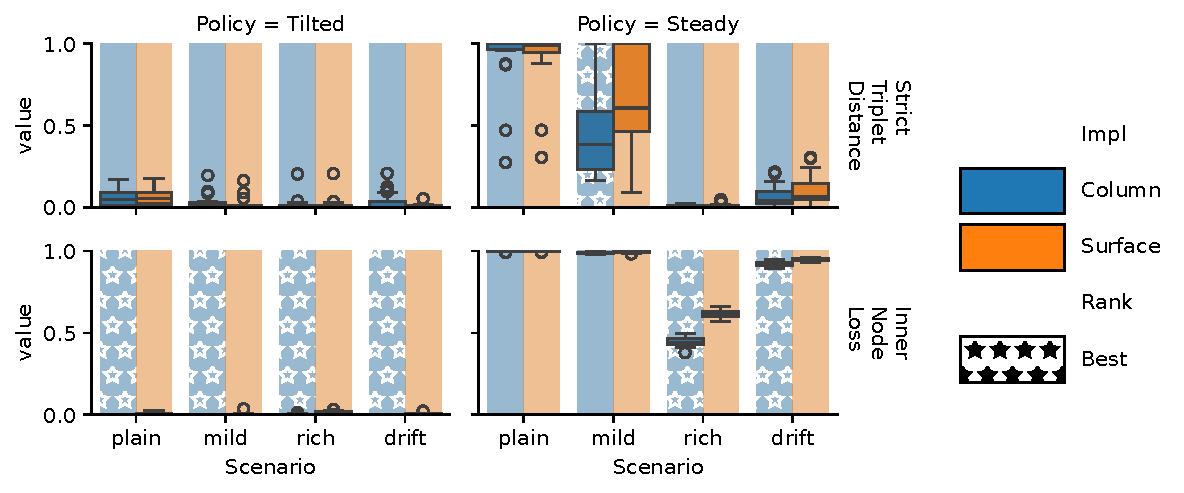
\includegraphics[width=\textwidth]{binder/binder/surf-vs-col/teeplots/annotation-size-bits=64+col=policy+differentia-width-bits=1+downsample=500+hue=impl+num-generations=100000+population-size=65536+post=teed-figure-subplots-adjust-right-0-72-teed-set-titles-row-templat.../e-row-name+row=variable+score=value+viz=peckplot+x=scenario+x-group=outer+y=value+ext=}
    \caption{Example reconstruction quality measure distributions. Lower is better.}
    \label{fig:col-vs-surf-example}
  \end{subfigure}%
  \begin{subfigure}[b]{0.5\textwidth}
    \centering
    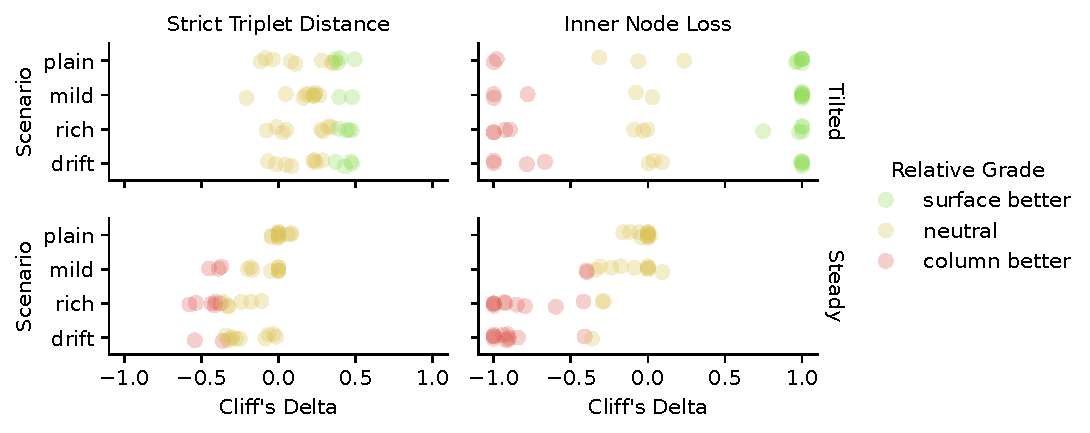
\includegraphics[width=\textwidth]{binder/binder/surf-vs-col/teeplots/col=metric+hue=relative-grade+kind=strip+post=teed-set-titles-col-template-col-name-row-template-row-name+row=policy+viz=catplot+x=cliff-s-delta+y=scenario+ext=}
    \caption{Reconstruction quality comparison outcomes.}
  \label{fig:col-vs-surf-overview}
  \end{subfigure}
  \caption{%
    \textbf{Does column- or surface-based instrumentation give higher-quality reconstruction?}
    Subpanel \ref{fig:col-vs-surf-overview} shows effect sizes of column-vs-surface comparisons for triplet distance and inner node loss metrics.
    Color coding indicates a significant outcome (Mann-Whitney U).
    Surface tends to outperform column under tilted policy and vice versa under steady policy.
    Subpanel \ref{fig:col-vs-surf-example} shows reconstruction quality effects for 64-bit size, bit-differentia annotations wit population size 65,536, downsample size 500, and 100k generations.
    Background hatching indicates significant outcome.
  }
  \label{fig:col-vs-surf-summary}
\end{figure*}


\begin{itemize}
    \item surf steady worse than col steady
    \item surf tilted better than col tilted
\end{itemize}

From this point onwards, only surf algorithms!!!

\subsection{Steady vs. Tilted} \label{sec:steady-vs-tilted}
\begin{itemize}
    \item steady worse than tilted
    \item hybrid similar to tilted
\end{itemize}

\begin{figure*}
  \centering
  \begin{subfigure}[b]{0.42\textwidth}
    \centering
    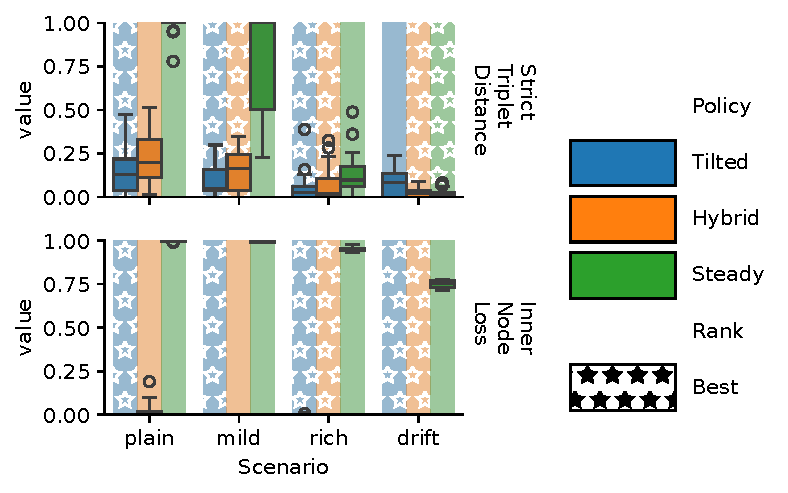
\includegraphics[width=\textwidth]{binder/binder/steady-vs-tilted/teeplots/annotation-size-bits=64+differentia-width-bits=1+downsample=500+hue=policy+num-generations=100000+population-size=65536+row=variable+score=value+viz=peckplot+x=scenario+x-group=outer+y=value+ext=}
    \caption{Example reconstruction quality distributions. Lower is better.}
    \label{fig:steady-vs-tilted-summary-example}
  \end{subfigure}%
  \begin{subfigure}[b]{0.58\textwidth}
    \centering
    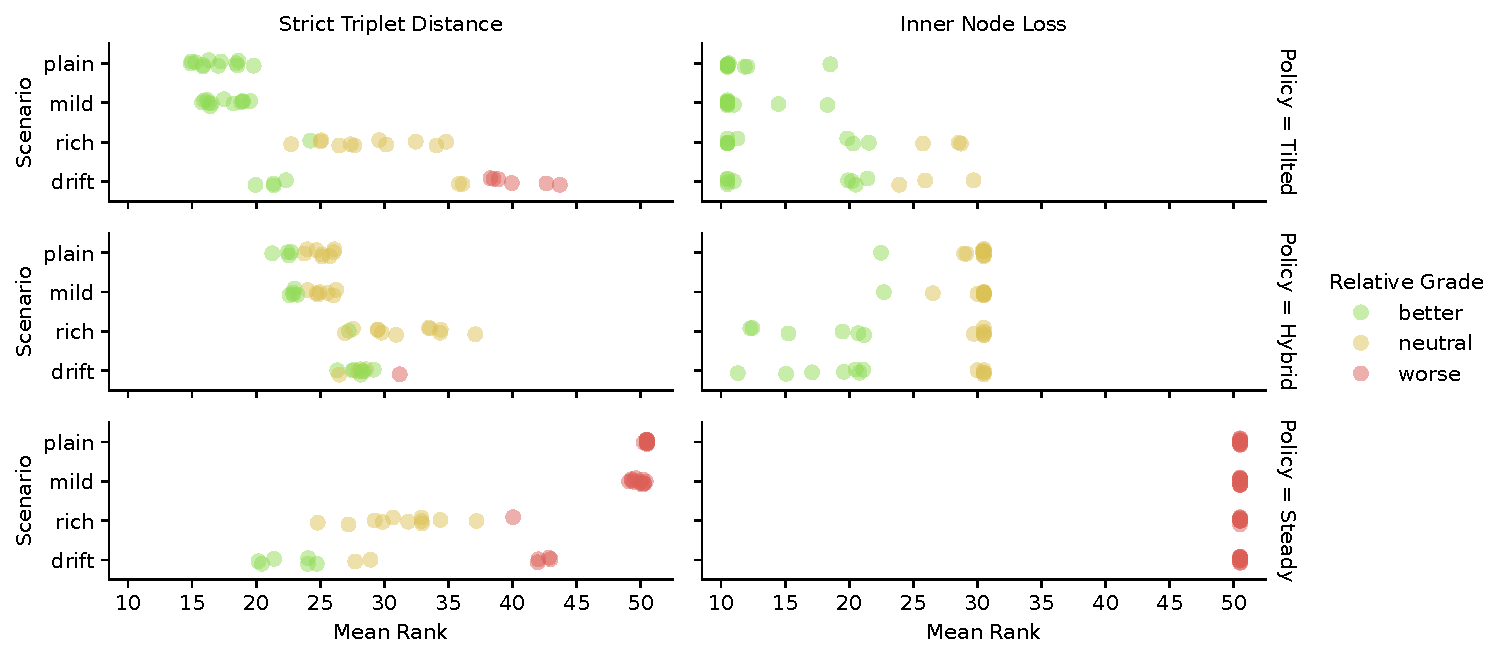
\includegraphics[width=\textwidth]{binder/binder/steady-vs-tilted/teeplots/col=metric+hue=relative-grade+kind=strip+row=policy+viz=catplot+x=mean-rank+y=scenario+ext=}
    \caption{Reconstruction quality comparison outcomes. Lower is better.}
    \label{fig:steady-vs-tilted-summary-overview}
  \end{subfigure}
  \caption{%
    \textbf{How does retention policy affect reconstruction quality?}
    \footnotesize
    Subpanel \ref{fig:steady-vs-tilted-summary-overview} shows mean rank among reconstruction error measures from tilted, hybrid, and steady retention policies across sensitivity analysis conditions.
    Each point represents an independent 20-replicate trial under different evolutionary conditions, instrumentation configuration (e.g., annotation size), and phylogenetic scale (e.g., reconstruction tip count).
    Color coding indicates significant outcome (Kruskal-Wallis H then Mann-Whitney U test).
    Lower is better.
    Tilted policy (top row) performs best in most evolutionary scenarios, except triplet distance under the highly phylogenetically-rich drift regime.
    Steady policy (bottom row) performs worst in most scenarios, except triplet distance under the drift regime.
    Hybrid policy performance has somewhat higher triplet distance reconstruction distance error in the plain and mild scenarios than tilted policy, but is robust to the drift regime.
    Subpanel \ref{fig:steady-vs-tilted-summary-example} shows reconstruction quality effects for 64-bit size, bit-differentia annotations with population size 65,536, downsample size 500, and 100k generations.
    Background hagching indicates significant outcome.
    See Supplementary Figure \ref{fig:steady-vs-tilted} for listing of reconstruction quality outcomes by sensitivity analysis condition \citep{moreno2024supplemental}.
  }
  \label{fig:steady-vs-tilted-summary}
\end{figure*}


\subsection{Why is Steady Bad? What Type of Error is Made?} \label{sec:error-analysis}
\begin{itemize}
    \item inner node loss from boxplot
    \item then, it's coming from recent nodes: node density vs. time histogram joyplot
    \item then, and that causes error: show error category (correct/wrong/unsure) vs. time stacked bar plot
\end{itemize}

From this point onwards, only surface-tilted (maybe also tilted-hybrid?) algorithm(s)!!!!

\subsection{Why are we seeing error? What can we do about it?} \label{sec:error-uncertainty}

mechanism of error: you have a lineage that diverges three ways between checkpoints (maybe make a figure of this); the two LEAST related happen to collide at the next checkpoint --- therefore, it looks like they're most related even though they're not.

sidebar: we can use differentia size to trade off between error and reconstruction accuracy; using 1 byte differentia essentially drives error to zero (but introduces uncertainty i.e., more polytomies in reconstruction)

\subsection{Does it Scale?} \label{sec:scaling}
% https://tex.stackexchange.com/a/159294/316176
\newcommand{\rulesep}{\unskip\ \vrule\ }

\begin{figure*}
  \centering
  \begin{subfigure}[b]{0.33\textwidth}
    \centering
    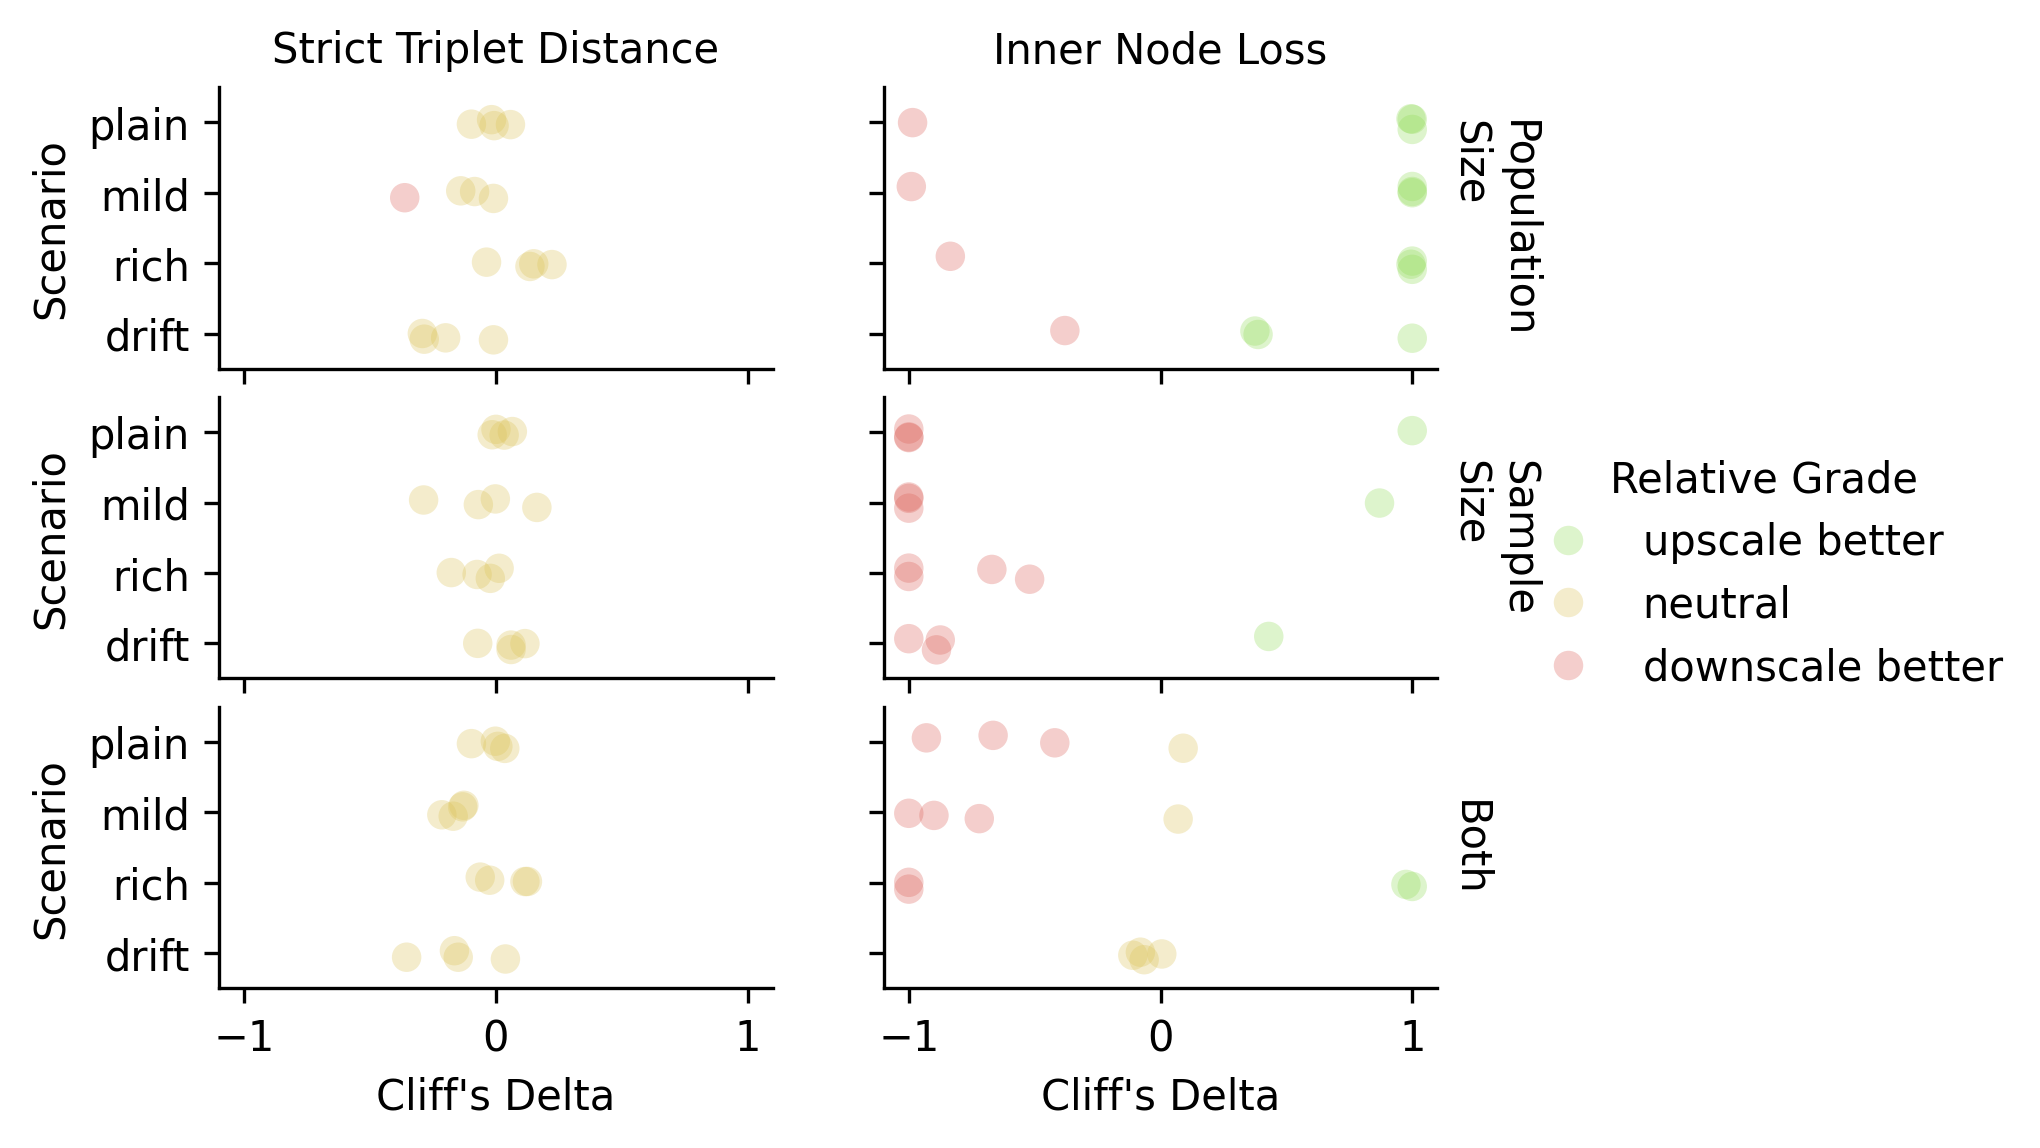
\includegraphics[height=1.7in,trim={0 0 5cm 0},clip]{binder/binder/dsamp-popsize-scale/teeplots/col=metric+hue=relative-grade+kind=strip+policy=tilted+row=scaling-factor+viz=catplot+x=cliff-s-delta+y=scenario+ext=}
    \caption{tilted retention policy (surface)}
  \end{subfigure}%
  \rulesep %
  \begin{subfigure}[b]{0.26\textwidth}
    \centering
    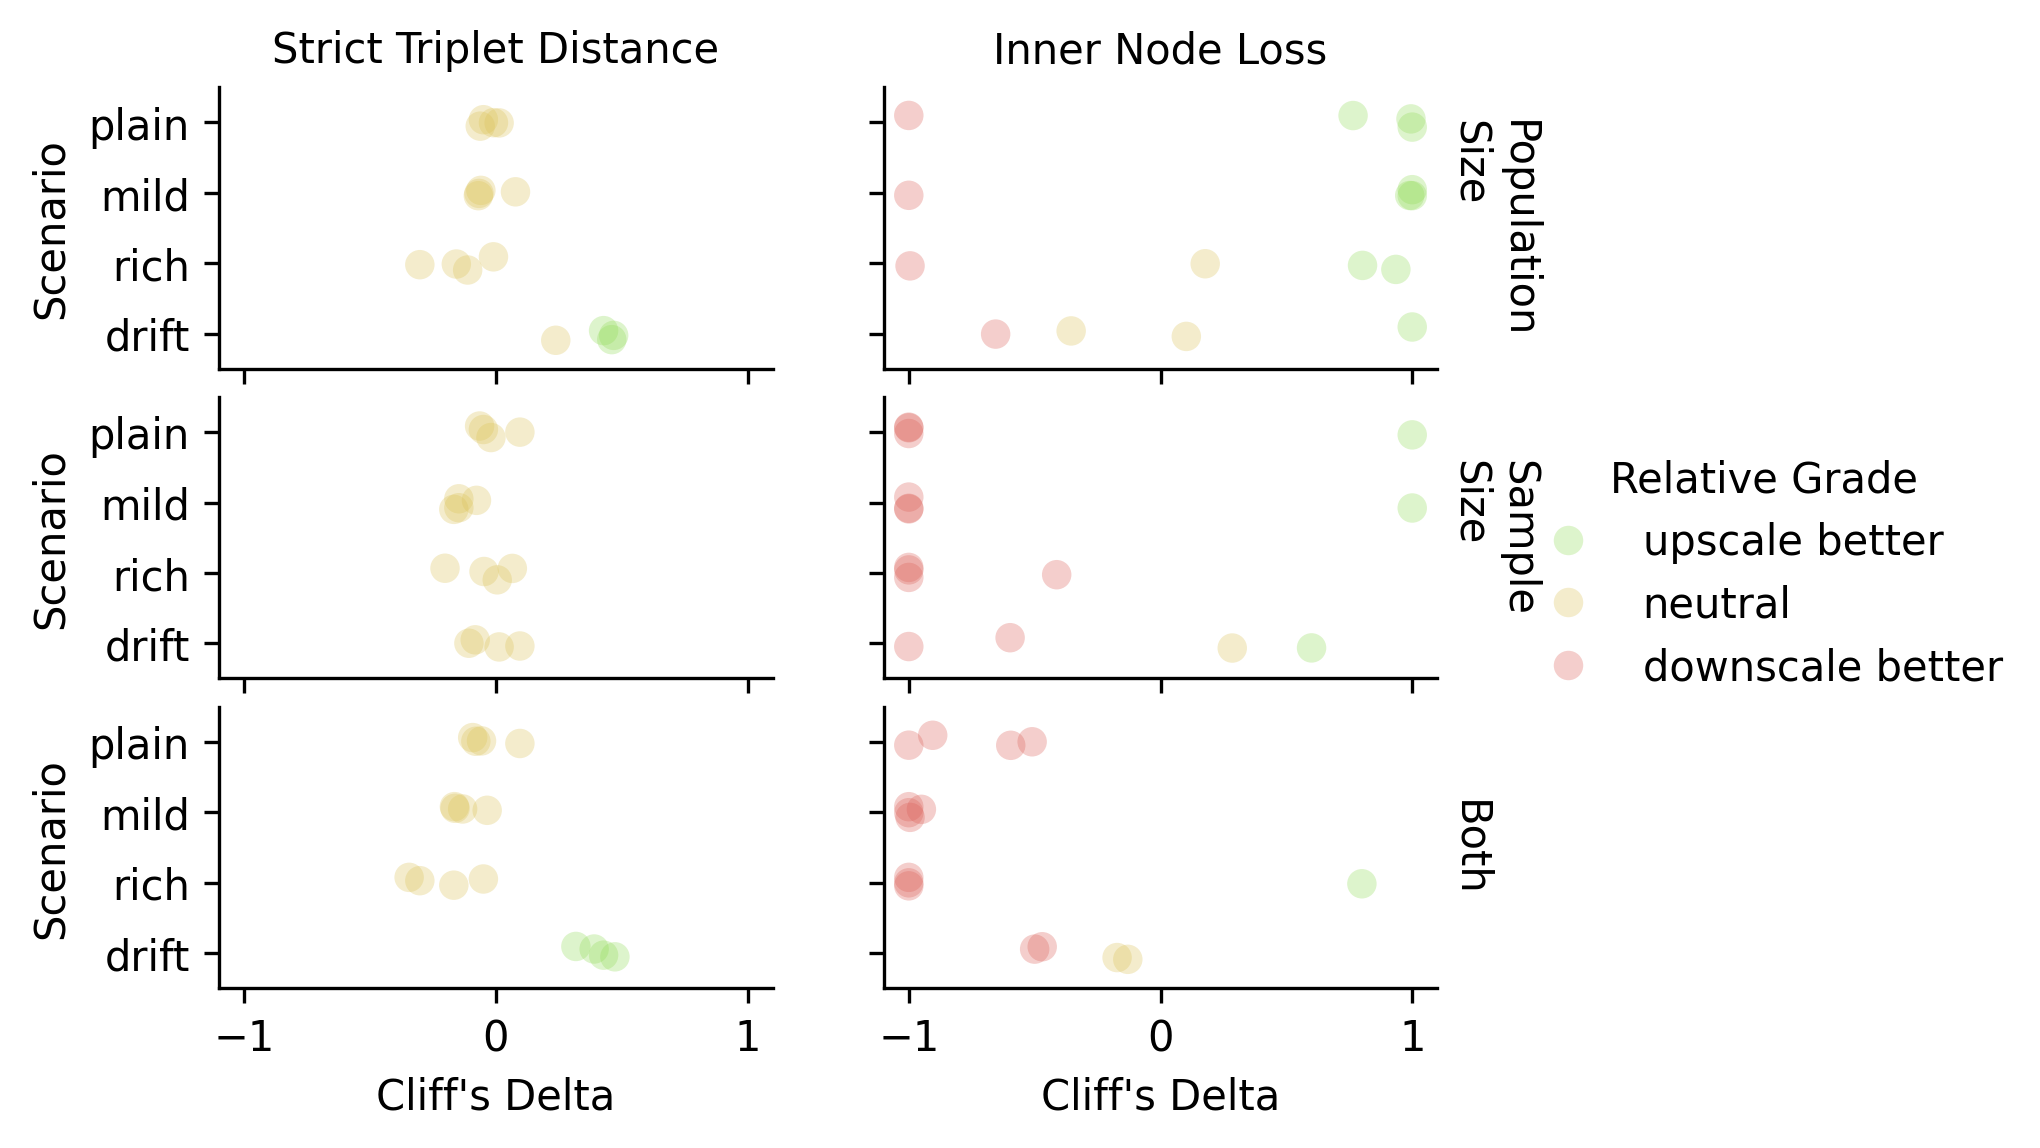
\includegraphics[height=1.7in,trim={2cm 0 5cm 0},clip]{binder/binder/dsamp-popsize-scale/teeplots/col=metric+hue=relative-grade+kind=strip+policy=hybrid+row=scaling-factor+viz=catplot+x=cliff-s-delta+y=scenario+ext=}
    \caption{hybrid retention policy (surface)}
  \end{subfigure}%
  \rulesep %
  \begin{subfigure}[b]{0.39\textwidth}
    \centering
    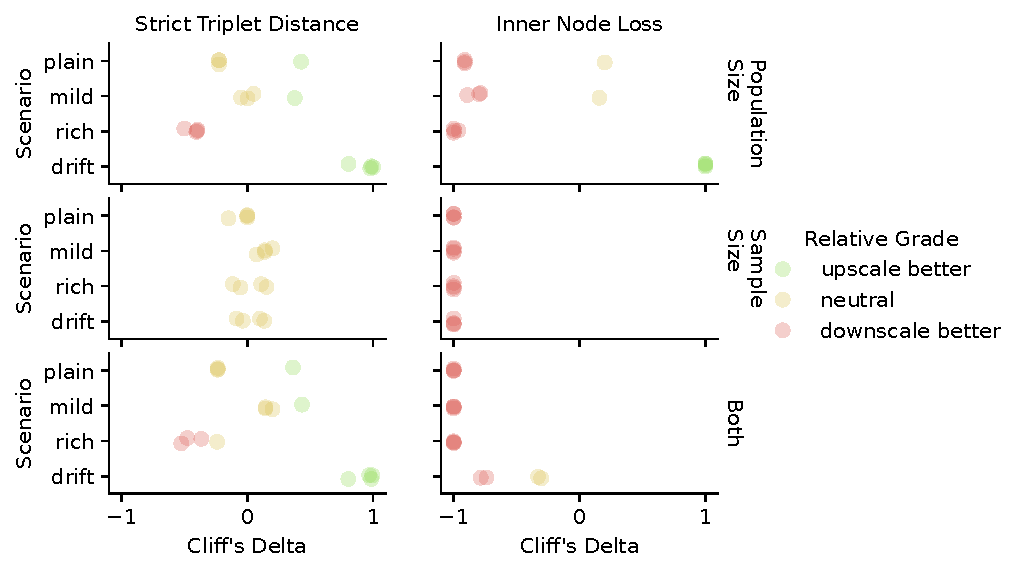
\includegraphics[height=1.7in,trim={2cm 0 0 0},clip]{binder/binder/dsamp-popsize-scale/teeplots/col=metric+hue=relative-grade+kind=strip+policy=steady+row=scaling-factor+viz=catplot+x=cliff-s-delta+y=scenario+ext=}
    \caption{steady retention policy (column)}
  \end{subfigure}
  \caption{%
  \textbf{How does scale impact reconstruction quality?}
  \footnotesize
  Each dot is a Cliff's Delta effect size of downscale-vs-upscale comparison under one sensitivity analysis condition.
  Color coding indicates a significant outcome (Mann-Whitney U).
  In order, rows show scaling outcomes for increasing population size, population subsample size (i.e., tree tip count), and both these factors.
  For tilted and hybrid policies, scaling had minimal effects on triplet distance and no systematic effect on inner node loss.
  Inner node loss worsened when scaling sample size, with and without scaling population size.
  Scaling effects were more variable under steady retention policy.
  See Supplementary Figures \labelcref{fig:dsamp-popsize-scale-hybrid,fig:dsamp-popsize-scale-steady,fig:dsamp-popsize-scale-tilted} for listing of effects by sensitivity analysis condition.
  }
  \label{fig:scaling-summary}
\end{figure*}


\begin{itemize}
    \item show reconstruction error and inner node count vs. pop size (error does not increase with pop size at fixed sample size)
    \item show reconst error/inner node count vs. time (error does not increase with time at fixed sample size)
    \item show reconst error/inner node count vs. sample size (error increases with sample size)
    \item show reconst error/inner node count vs. bit size at large sample (we can reduce the error for large sample size by increasing bit size)
\end{itemize}

\subsection{Synthesis} \label{sec:synthesis}

\textbf{Algorithm Configuration}
\begin{itemize}
\item \textbf{Direct tracking or reconstruction-based approach?}
  In highly parallel and distributed experiments, reconstruction-based approach (hereditary stratigraphy) provide simpler implementation, lower runtime overhead costs, and greater robustness to data loss.
  In serial or centralized simulations, direct phylogenetic tracking should usually be preferred due to its capability for perfect record-keeping.
  However, reconstruction-based tracking may have certain advantages in some circumstances: under requirements for hard limits on memory use, hard real time operation, or where agents are frequently serialized/stored between different experiments and being able to retain their phylogenetic histories without keepin a global phylogenetic record is desirable.
\item \textbf{Retention policy: steady or tilted?} 
  If you suspect \textit{very weak} phylodiversity-enhancing factors (ecology, spatial structure, low seletion pressure), use a steady policy.
  If you expect strong phylodiversity-enhancing factors or are unsure, use a hybrid policy or a tilted policy.
  In rare cases where phylodiversity-enhancing factors are very strong (e.g., pure drift conditions), a tilted policy may be appropriate.
  Suggested default choice: hybrid policy.
\item \textbf{Differentia size: bit or byte?}
  Bit-size differentia maximize the fraction of correct reconstruction outcomes, but can also introduce incorrect reconstruction outcomes.
  Byte-size differentia have very low incorrect reconstruction outcome rates, but have a larger incidence of unresolved reconstruction oucomes (false polytomies).
  If you need very strong guarantees against incorrect reconstruction outcomes, an even larger differentia size (32 or even 64 bits) may be appropriate. 
  Suggested default choice: bit-size differentia.
\item \textbf{Annotation size: constant or dynamic?}
  In most scenarios, a constant-size annotation will be more computationally efficient and ensure fuller use of available memory resources.
  However, if you need hard guarantees on recency-proportional inference quality, use a annotation size that scales $\mathcal{O}log(n)$ with generational depth.
  Suggested default choice: constant-size annotations.
\item \textbf{Annotation size: how many bits?}
  This factor trades off between memory-use and communication-bandwidth overhead for annotations and quality of reconstructed phylogenies.
  In cases where annotation size is not a limiting factor, when using single-bit differentia 256 bit annotations will discern phylogenetic events with about 13\% recency-relative precision (tilted) or 1\% depth-relative precision (steady) through 1 billion generations.
  For full-byte differentia, an annotation size on the order of kilobits would be very robust.
  Where annotation resource use is a limiting factor, a 64 bit annotation can give good results.

  Current implementations of surface algorithms are limited to buffer sizes that are even powers of two (32, 64, 128, etc.).
  Where finer gradations are desired, intermediate differentia sizes (e.g., storing 3 bit differentia over 32 surface sites would occupy 96 bits) or alternating depositions onto amalgamated surfaces might be considered (e.g., a 32 bit tilted surface and a 16 bit steady surface) --- although the latter would require some minor algorithm implementaiton customizations akin to those conducted for the hybrid surface.
  Column algorithms are more flexible in buffer sizing, but make less full use of available buffer space.

  According to results here, simulation scale does not appear to be a major factor in considering annotation size, because at the same absolute sample sizes samples from differently sized populations have no clear trend in reconstruction quality characteristics.
  However, sample size may play into decision of annotation size (see below).

  Note that in addition to differentia values, a generation counter will also need to be stored in genomes (for most use cases, a 32- or 64-bit value).

  In scenarios where explicitly differentiating between founding clades is paramount, 
  \footnote{One possible exception is cases where a global monotonic counter is available and it is desirable to demarcate phylogenetic history in terms of simulation time rather than generations.}
\item \textbf{Implementation: column or surface?}
  If you are using dynamic annotation size, you will need a column-based implementation to allow differentia count fluxuations.
  Otherwise, for constant annotation size, surface implementations are much more efficient \citep{TODOOTHERPAPER}.
  In the case of tilted retention policy, they also give higher-quality reconstructions.
  If using steady policy, column implementation gives higher-quality reconstructions and is preferable if computational performance is not a concern.
  Another factor that might influence this decision is the software platform being designed for.
  If packages providing hereditary stratigraphy are not available, surface algorithms are easier to implement owing to greater orthogonality between the algorithm implementaiton (site selection) and data structure (simple buffer).
  Suggested default choice: surface implementation.
\item \textbf{Administration: update frequency?}
  For most applications, hereditary stratigraph updates should correspond directly to generations elapsed.
  However, in cases with expected very high generation counts that outstrip the capacity of on-genome counter size and fine-resolution visibility over recent history is not necessary.
  In other circumstances, where time-indexed resolution is preferred or ultrametricity (even branch lengths from root) is paramount, it may be preferred to update annotations on the basis of simulation update cycles rather than generations.
  Under this approach, annotations on all genomes
  Suggested default choice: every-generation updates.
\item \textbf{Simulation content: sexual or asexual?}
  The core of existing hereditary stratigraphy is designed around asexual lineages and that makes it very straightforward and simple to apply to evolution simulations with asexual reproduction.
  Although there has been some preliminary work demonstrating applications of hereditary stratigraphy to sexual populations, operating procedures are not as well developed for this mode of evolution.
  One possibility includes tracking asexual lineages of individual genes (``gene trees'').
  Organism-level annotation could be used to track the emergence of new independently-breeding subpopulations (``species trees''').
  This approach relies on distinct annotation values reaching fixation within independent subpopulations.
  This can be accomplished through drift where offspring inherit the differentia record of a randomly-selected parent or, alternatively, through a gene drive mechanism where, for many-bit differentia, large-magnitude values are favored for inheritance and thereby rapdily sweep through interbreeding subpopulations. 
  Refer to \citep{moreno2024methods} for additional discussion.
\item \textbf{Sampling strategies}
Care will need to be taken to account for sample size and sample size relative to the whole population in analyses.
Triplet distance appears to be largely stable under surveyed increases in sample size.
However, loss of inner nodes occuring near the tips is observed when increasing sampling size.
Where this is a problem, differentia count and/or size should be increased.

Note that reconstruction techniques are fully compatible to stitch together across widely-varying time points.
Indeed, these taxa can provide valuable information about extincted lineages.
Intermediate taxa can sould serve a role akin to ``fossils'' in studies of natural history.

For more advanced analyses, it may be desirable to associate sampled strata with trait data \citep{TODOMODES,TODOCITEFROMJACOB}

\end{itemize}

\textbf{Simulation Integration}

Three major steps will be necessary to be implemented to run the hereditary stratigraphy pipeline: (1) integration of instrumentation into the simulation runtime genome model, (2) serialization of evolved agents' markers from simulation, (3) loading data into the Python \textit{hstrat} library in order to analyze it.

\begin{itemize}
\item \textbf{Runtime Annotations}: 
You will need to augment the Genome data structure in your simulation code in two ways: (1) to store hereditary stratigraphic annotation data and (2) add a call to the copy/reproduce or mutate function to update the differentia store and bump the generation counter.

For sufaces, two components are required: a fixed-buffer differentia store and a generation counter.
The differentia store can be implemented as an array of integer data types (e.g., \texttt{uint8}), but for bit differentia you will likely want to use a raw memory array or an abstraction around it if available (e.g., \texttt{std::bitset}).

Surfaces also have a simple update procedure.
Call \texttt{pick\_deposition\_site} and randomize the differentia element at the returned nth position.

Software implementing column-based approaches is available for Python \citep{moreno2022hstrat} and surface-based approaches are available for Python \citep{TODO}, and Zig/Cerebras Software Language \citep{TODO}.
Based on community feedback, C/C++ and Rust are priority targets to port hstrat surface implementations to.

If you are using another software language, porting core algorithms should be doable with moderate effort.
Are implemented primarily as a library of small functions ($\approx<30$ LOC) with accompanying tests, making them amenable to stepping-stone piece by piece transliteration.
We found LLM assistance to be highly effective in translating the surface algorithms from Python to Zig \citep{TODO}.
Feel free to get in touch --- we would be happy to furnish these algorithms in other languages if you have a use case.
\item \textbf{Serialization}
In order to transfer marker data for postprocessing, you will need to save it to file.
For best compatibility with the analysis pipeline, extract annotations and save them together in a conventional format separate from other genome components (e.g., JSON, CSV).
For each annotaiton, you will need to store the generation counter and the differentia data.
One convenient plain text way to encode differentia data is as a hex string.

In order to conduct postprocessing, you will need to use tools in the \textit{hstrat} library.
When reserializing the data, you will need to know the 11¡retention policy and differentia width used so make sure these are recorded somewhere.
Functions to convert raw data into intantiated \texttt{Column} objects are described in package documentation and examples, with a variety of entry points compatible with JSON, YAML, and CSV formats. 

Note that, while the hstrat library also provides support to deserialize from compact binary formats in many circumstances, storage in plain text format with zipping (e.g., gzip) will provide competitive --- if not better --- space efficiency to binary representations and can be considerably easier to work with.

\item \textbf{Analysis}
Reconstruction algorithms are currently implemented in the \textit{hstrat} library.
This algorithm takes a list of deserialized column objects and produces a phylogeny.
Optionally, a list of taxa identifiers may also be provided if desired.
A variety of tools for estimation of MRCA between marker pairs or groups are also provided.
Reconstructions are reported in alife community data standard format \citep{TODO}.
Tools are provided that can convert these formats to standard bioinformatics formats for interoperation with the rich existing software ecosystem for phylogenetic visualization and analysis \citep{TODOalifedataphyloinformaticsconvert}.
\end{itemize}

Our goal in building the software for hereditary stratigraphy is to provide sufficient documentation and convenient APIs to constitute a plug-and-play add-on that can be taken off the shelf with minimal effort.
Building a user base is a key priority for the project, and we would be very interested in collaborating to integrate hereditary stratigraphy instrumentation into your system or provide algorithm implementations for your particular runtime.

